\documentclass[10pt,oneside,onecolumn,letterpaper]{article}
\usepackage{graphicx}
\usepackage{xcolor}
\usepackage[hidelinks]{hyperref}
\usepackage{booktabs}
\usepackage{adjustbox}

\usepackage[top=.5in, bottom=1in, left=.5in, right=.7in]{geometry}

\usepackage{fontspec}
\setmainfont{Arial}

\begin{document}

%%
% THIS IS THE HEADER
%%
\noindent\colorbox{black}{
\begin{minipage}[c]{.99\linewidth}
  \vspace{.4cm}
  \Large{\color{white}{\textbf{\hspace{.3cm}University of Massachusetts Boston}}}
  \begin{flushright}
    \vspace{-1.2cm}
    
\includegraphics[width=3cm]{gfx/cs460.png}
  \end{flushright}
\end{minipage}
}

%%
% CONTENT STARTS HERE
%%

\vspace{.5cm} % add some space

\noindent\textbf{CS460 Fall 2019} \\
\textbf{Name:} Jared Barresi \\
\textbf{Student ID:} 00974358 \\
\textbf{Due Date:} 11/27/2019

\section*{Assignment 9: Geometry, Materials, and Lighting!}

\textbf{We will load our favorite mesh from a file, try out different materials, and play around with light settings.}

\vspace{.5cm} % add some space

\begin{center}
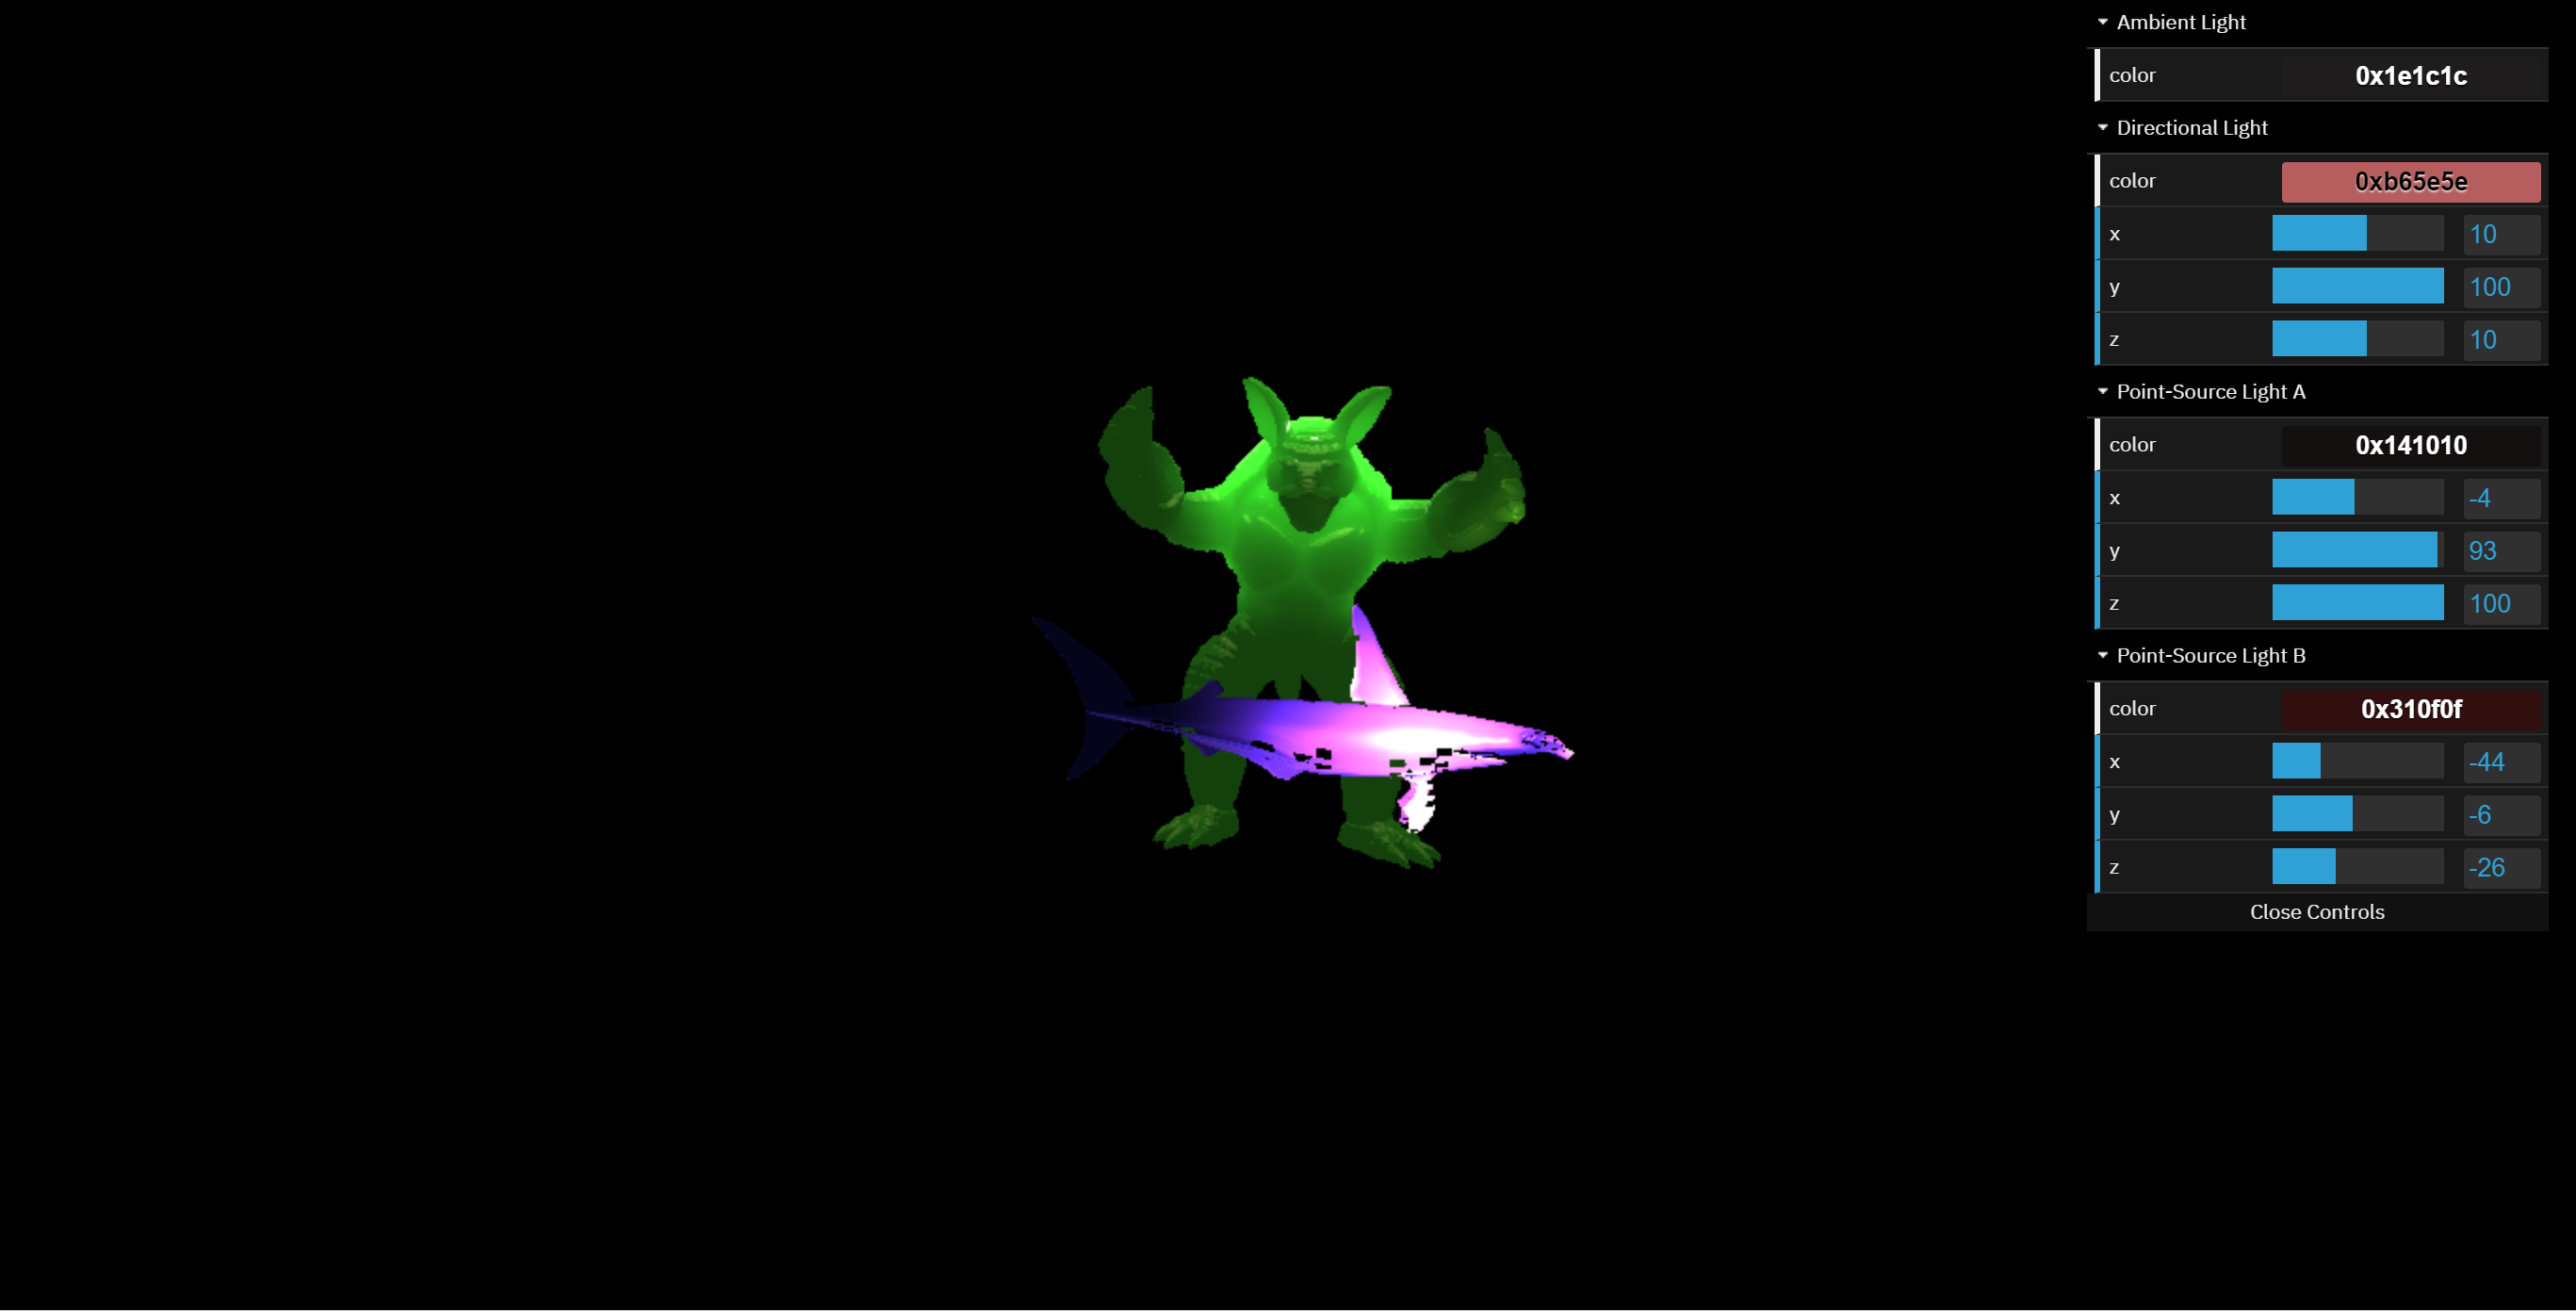
\includegraphics[width=.5\textwidth]{gfx/screenshot-1.png}
\end{center}

\vspace{.5cm}

\noindent\textbf{Starter code for assignment 9.} After pulling from upstream, there is the folder \url{09} in your fork. If you run a webserver and access the file, you will see a sad single armadillo in the scene.

\vspace{.5cm}


\noindent\textbf{Part 1 (14 points):} The armadillo needs a friend! Please load a second mesh from a file using a THREE.js loader. This could be any mesh you find online in any format THREE.js supports - or you could load the armadillo again. Please modify the positions so that the meshes do not overlap.

\vspace{.5cm}

\noindent\textbf{Part 2 (15 points):} Please configure the second mesh from above with a different material of your choice (not MeshToonMaterial again!).

\vspace{.5cm}

\noindent\textbf{Part 3 (10 points):} Please add two point light sources to the scene.

\vspace{.5cm}

\noindent\textbf{Part 4 (15 points):} The starter code includes the following snippet to control the color and position of the directional light.

\begin{verbatim}
var directionalFolder = gui.addFolder('Directional Light');
directionalFolder.addColor(controller, 'color').onChange( function(value) {
  directionalLight.color.setHex(value); 
});
directionalFolder.add(directionalLight.position, 'x', -100, 100);
directionalFolder.add(directionalLight.position, 'y', -100, 100);
directionalFolder.add(directionalLight.position, 'z', -100, 100);
directionalFolder.open();   
\end{verbatim}

Please setup dat.GUI to control position and color of the two point lights with similar code.

\vspace{.5cm}
\newpage
\noindent\textbf{Part 5 (15 points):} Please setup dat.GUI to control the color of both materials.


\vspace{.5cm}
\noindent\textbf{Part 6 (30 points):} Please play around with the lights and try to understand why the toon material seems to work *sometimes*. What are your observations?

\vspace{.5cm}

\noindent{The mesh disappears if the source lights are completely black. If they are the same color as the mesh color, the textures (which are made visible by shadows) are no longer visible. \newline \newline Also, if you turn off all but the point source lights, the portion of the meshes that are in the path of the point source lights follow the same pattern as above, however it also creates a sort of "glowing" effect on the mesh the point source comes in contact with.\newline \newline In addition, I was able to get some interesting effects by modifying the intensity and distance settings of the point source lights. }

\vspace{3cm}

\noindent\textbf{Part 9 (1 points):} Please update the screenshot above with your own and then post the github pages url here:

\vspace{.5cm}

\url{https://hltdev8642.github.io/cs460student/09/index.html}

\vspace{3cm}

\newpage

\noindent\textbf{Bonus (33 points):}

\vspace{.5cm}

\noindent\textbf{Part 1 (11 points):} Please add dat.GUI elements that allow to switch the material for the two meshes. Here is an example of a combobox in dat.GUI:

\vspace{.5cm}

\begin{verbatim}
// Choose from accepted values
gui.add(controller, 'material', [ 'toon', 'standard', 'phong' ] ).onChange( function(value) {
  
  if (value == 'phong') {
    // TODO
  }

});
\end{verbatim}

\vspace{.5cm}

\noindent\textbf{Part 2 (22 points):} Please make adding lights to the scene dynamic: Add dat.GUI buttons to add new directional lights that then also add a dat.GUI folder to the menu that allows to control (color and position), and remove the light.

\end{document}
